% rosetta/appendix-flow.tex — 附录 B：KW06 逻辑流程图
\section{KW06 的逻辑流程}
\label{app:flow}

下图把论文十二节的论证骨架压成一张图：左栏是物理侧的输入（4 维 $\mathcal N=4$ 超对称杨--米尔斯、$S$-对偶、拓扑扭化），右栏是数学侧的产物（Hitchin 模空间、A/B 膜、$\mathcal D$-模、Hecke 特征层），中间是两条主干：一条把扭化后的规范理论化为 Hitchin 模空间上的拓扑场论，另一条把膜范畴与 $\mathcal D$-模范畴对应起来，最终给出几何 Langlands 对应的物理证明框架。

\clearpage

\newgeometry{left=1.0cm,right=1.0cm,top=1.0cm,bottom=1.0cm}
\begin{landscape}
\thispagestyle{plain}
\vspace*{0.2cm}
\begin{center}
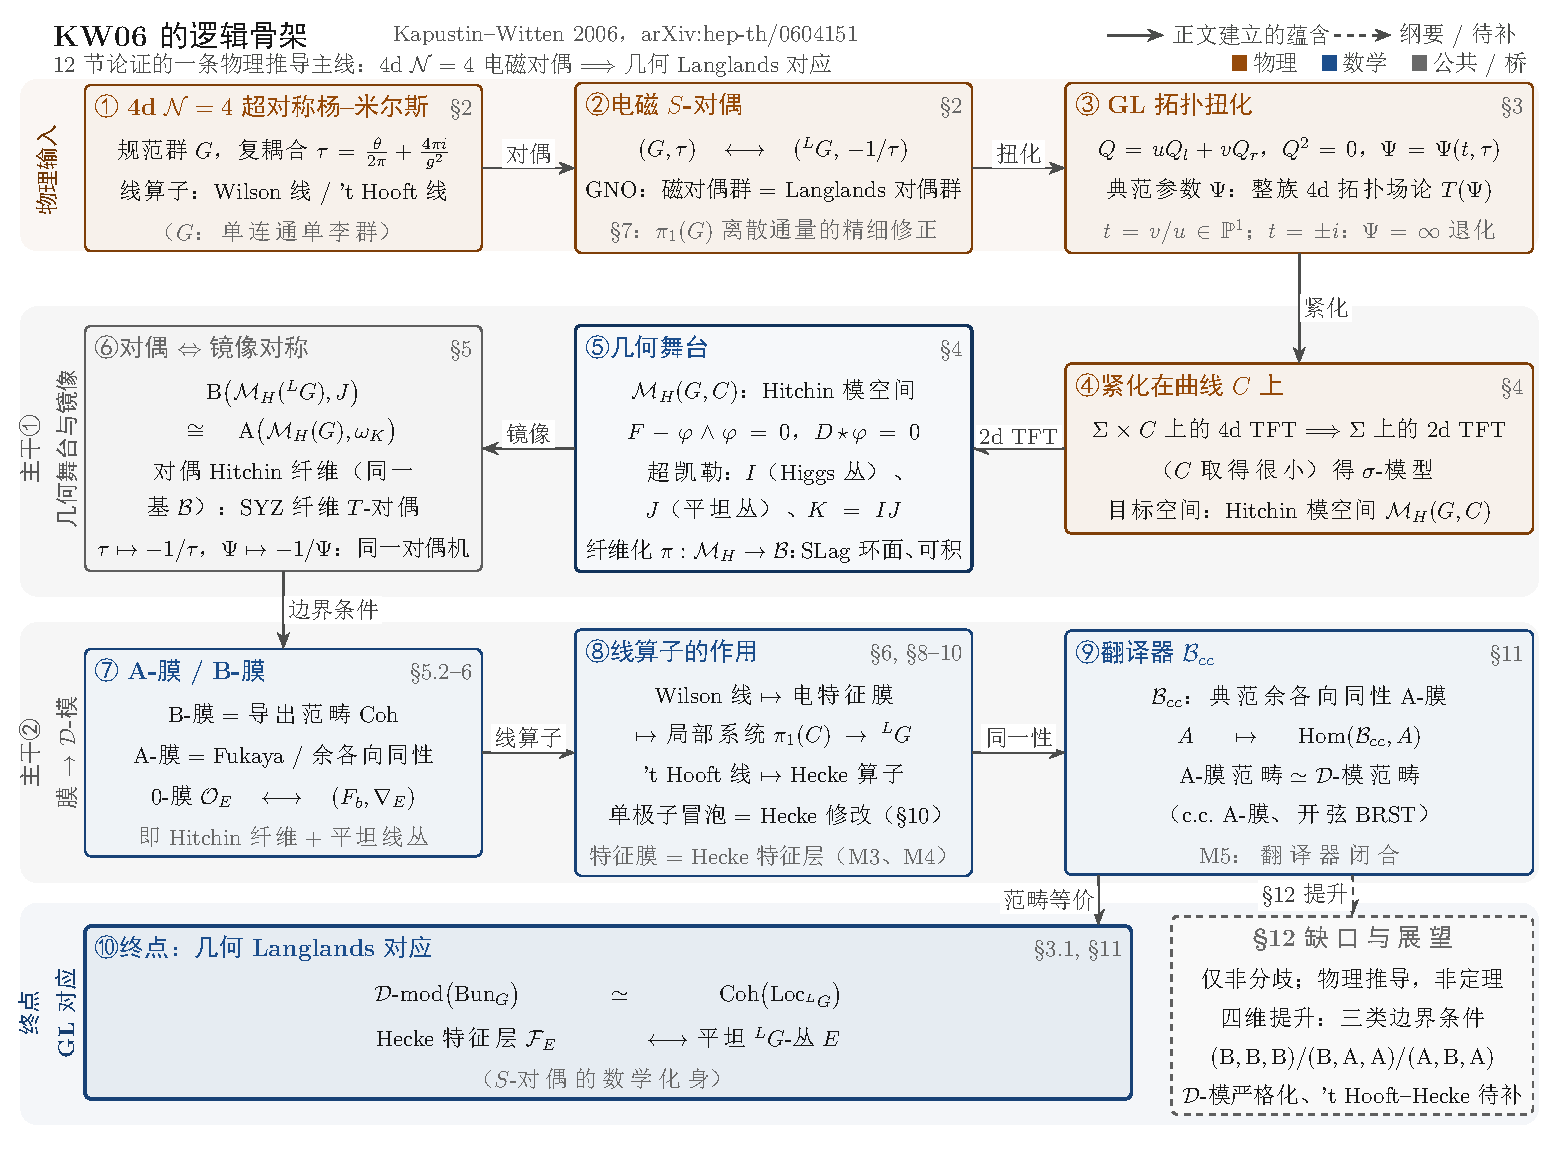
\includegraphics[width=0.92\linewidth,height=0.86\textheight,keepaspectratio]{flow/flow.pdf}
\end{center}
\vspace{0.15cm}
\noindent{\small\color{gcol}读图方式：从上往下读是「物理输入 $\to$ 数学结构」；从下往上读是「数学命题 $\to$ 物理实现」。实线箭头表示正文明确建立的蕴含，虚线箭头表示 KW06 只给论证纲要、细节留待后续的地方。}
\end{landscape}
\restoregeometry
